\documentclass[
    style=OCRALevel,
    coverstyle=WellyOCR
]{examx}

\printanswers

\examtitle{L6th FM Mechanics Assessment}
\examdate{LT 2022}
\examtime{50 minutes}

% This exam is questions 9-13 of H240/03 Pure Mathematics and Mechanics Sample Question Paper. Q4 has been modified, Q2 has been replaced.

\begin{document}
	\examcover
	\begin{questions}
		\question
		Two forces, of magnitudes $\qty{2}{\N}$ and $\qty{5}{\N}$, act on a particle in the directions shown in the diagram 
		below.		
		
		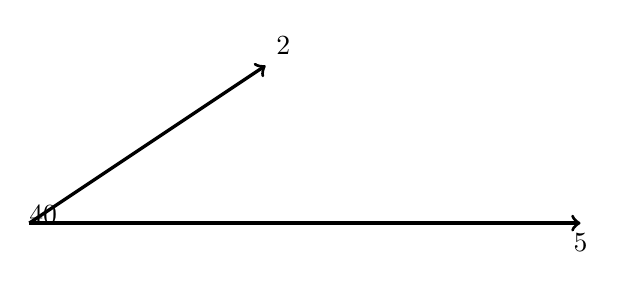
\begin{tikzpicture}
			\coordinate (O) at (0,0);
			\coordinate (A) at (7,0);
			\coordinate (B) at (3,2);
			
			\draw[very thick,->] (O)--(A) node[pos=1,below]{$\qty{5}{\N}$};
			\draw[very thick,->] (O)--(B) node[pos=1,above right]{$\qty{2}{\N}$};
			
			\tkzMarkAngle[mark=none](A,O,B);
			\tkzLabelAngle[pos=1.5](A,O,B){$40\degree$};
		\end{tikzpicture}
		\begin{parts}
			\part[3][5] Calculate the magnitude of the resultant force on the particle.
			
			\part[1][3] Calculate the angle between this resultant force and the force of magnitude $\qty{5}{\N}$.
		\end{parts}
		
		\solnor{
			\begin{parts}
				\part Attempt resolution of forces (allow $\sin$ and $\cos$ confusion) \exmark[M1] \\
				Horizontal component $=5+2\cos40$ and/or vertical component $=2\sin40$ \exmark[A1] \\
				$\sqrt{6.5321^2+1.2856^2}=\qty{6.66}{\N}$. \exmark
				\part $\tan^{-1}(\frac{2\sin40}{5+2\cos40})=11.1\degree$ \exmark[B1FT]
			\end{parts}
		}
        \solnpage
		
%		\question
%		A body of mass $\qty{20}{\kg}$ is on a rough plane inclined at angle $\alpha$ to the horizontal.
%		
%		The body is held at rest on the plane by the action of a force of magnitude $P\,\unit{\N}$.
%		
%		The force is acting up the plane in a direction parallel to a line of greatest slope of the plane.
%		 
%		The coefficient of friction between the body and the plane is $\mu$.
%		
%		\begin{parts}
%			\part[4][15] When $P=100$, the body is on the point of sliding down the plane.
%			
%			\bigskip
%			Show that $\grav \sin\alpha=\grav\mu\cos\alpha+5$.
%			
%			\part[3][15] When $P$ is increased to 150, the body is on the point of sliding up the plane.
%			
%			\bigskip
%			Use this, and your answer to part {\bfseries(a)}, to find an expression for $\alpha$ in terms of $\grav$.
%		\end{parts}
%	
%		\solnor{
%			\begin{parts}
%				\part Diagram or equivalent explanation including reaction, $\qty{100}{\N}$ force, friction, and weight \exmark[B1]:
%				
%				\begin{tikzpicture}
%					\coordinate (O) at (0,0);
%					\coordinate (A) at (6,0);
%					\coordinate (B) at (8,4);
%					\coordinate (P) at (4,2);
%					\coordinate (P1) at ($(P)+(-0.2,0.2)$);
%					\coordinate (R) at ($(P1)+(-1,2)$);
%					\coordinate (F) at ($(P1)+(2,1)$);
%					\coordinate (W) at ($(P1)+(0,-2)$);
%					
%					\draw[very thick, dashed] (O)--(A);
%					\draw[very thick] (O)--(B);
%					\fill (P1) circle (0.282);
%					\draw[very thick,->] (P1)--(R) node[pos=1,above left]{$R$};
%					\draw[very thick,->] (P1)--(F) node[pos=1,above left]{$\qty{100}{\N}+F$};
%					\draw[very thick,->] (P1)--(W) node[pos=.5,right]{$20\grav\,\unit{\N}$};
%					
%					\tkzMarkAngle[mark=none](A,O,B);
%					\tkzLabelAngle[pos=1.5](A,O,B){$\alpha$};
%				\end{tikzpicture}
%			
%				Resolve parallel to the slope \exmark[M1]:
%				\begin{equation}\label{eq:parallel}
%					100+F-20\grav\sin\alpha=0
%				\end{equation}
%			
%				Resolve perpendicular to the slope and note that friction is maximum \exmark[M1]:
%				\begin{equation*}
%					R=20\grav\cos\alpha \text{ and } F=\mu R
%				\end{equation*}
%			
%				Substitute to obtain the result \exmark[E1]
%				\begin{align*}
%					20\grav\sin\alpha&=F+100 \\
%					&=\mu R+100 \\
%					&=20\grav\mu\cos\alpha+100
%				\end{align*}
%				\part Diagram or equivalent explanation including reaction, $\qty{100}{\N}$ force, friction, and weight \exmark[B1]:
%				
%				\begin{tikzpicture}
%					\coordinate (O) at (0,0);
%					\coordinate (A) at (6,0);
%					\coordinate (B) at (8,4);
%					\coordinate (P) at (4,2);
%					\coordinate (P1) at ($(P)+(-0.2,0.2)$);
%					\coordinate (R) at ($(P1)+(-1,2)$);
%					\coordinate (F) at ($(P1)+(2,1)$);
%					\coordinate (W) at ($(P1)+(0,-2)$);
%					\coordinate (PF) at ($(P1)+(-2,-1)$);
%					
%					\draw[very thick, dashed] (O)--(A);
%					\draw[very thick] (O)--(B);
%					\fill (P1) circle (0.282);
%					\draw[very thick,->] (P1)--(R) node[pos=1,above left]{$R$};
%					\draw[very thick,->] (P1)--(F) node[pos=1,above left]{$\qty{150}{\N}$};
%					\draw[very thick,->] (P1)--(PF) node[pos=1,above left]{$F$};
%					\draw[very thick,->] (P1)--(W) node[pos=.5,right]{$20\grav\,\unit{\N}$};
%					
%					\tkzMarkAngle[mark=none](A,O,B);
%					\tkzLabelAngle[pos=1.5](A,O,B){$\alpha$};
%				\end{tikzpicture}
%			
%				Resolve parallel to the slope \exmark[B1]:
%				\begin{equation}\label{eq:paralleltwo}
%					150-F-20\grav\sin\alpha=0
%				\end{equation}
%			
%%				From \eqref{eq:parallel} and \eqref{eq:paralleltwo} \exmark[M1]
%				\begin{equation*}
%					250-40\grav\sin\alpha=0
%				\end{equation*}
%				so \exmark[A1]
%				\begin{equation*}
%					\alpha=\sin^{-1}\frac{25}{4\grav}
%				\end{equation*}
%			\end{parts}
%		}

%New question
%		\question
%		A body of mass $\qty{8}{\kg}$ is on a rough horizontal plane acted on by a force $P\,\unit{\N}$ at angle $\alpha$ above the horizontal.
%		
%		\begin{parts}
%			\part[1][4] Write down an expression for friction $F$ in terms of $P$ and $\alpha$.
%			\part[2][8] The coefficient of friction between the body and the plane is $\mu$ and the body is on the point of sliding.
%			
%			Show that $F=8\mu \grav-\mu P\sin\alpha$.
%		\end{parts}
%		
%		\bigskip
%		From now on, $P=10\grav$ and $\alpha$ is such that $\sin\alpha=3/5$ and $\cos\alpha=4/5$.
%		\begin{parts}
%			\setcounter{partno}{2}
%			\part[2][4] Find the value of $\mu$
%			\part[2][6] The angle $\alpha$ is now reduced to zero, does the body move?
%		\end{parts}
%	
%		\solnor{
%			\begin{parts}
%				\part $F=P\cos\alpha$ \exmark
%				\part $R=8\grav-P\sin\alpha$ \exmark[M1] so $F=8\mu \grav-\mu P\sin\alpha$ \exmark
%				\part $8\mu\grav-6\mu\grav=8\grav$ \exmark[M1] so $\mu=4$
%				\part $R=8\grav$ so $F_{\max}=32\grav>10\grav$ \exmark[M1] so the body does not move \exmark
%			\end{parts}
%		}

		\question[8][20]
		A box of mass $\qty{30}{\kg}$ is being pulled along rough 
		horizontal ground at a constant speed using a rope. The rope 
		makes an angle of $20\degree$ above the ground. The coefficient 
		of friction between the box and the ground is $0.4$. The rope 
		is modelled as an inextensible string. what is the tension in 
		the rope?
        
        \solnor{TBD}
		
		\examnewpage
		\question
		In this question the unit vectors $\vec{i}$ and $\vec{j}$ are in the directions east and north respectively.
		
		\bigskip
		A particle of mass $\qty{0.12}{\kg}$ is moving so that its position vector $\vec{r}$ metres at time $t$ seconds is given by $\vec{r}=2t^3\vec{i}+(5t^2-4t)\vec{j}$.
		\begin{parts}
			\part[3][6] Show that when $t=0.7$	the bearing on which the particle is moving is approximately $044\degree$.
			\part[4][8] Find the magnitude of the resultant force acting on the particle at the instant when $t=0.7$.
			\part[2][6] Determine the times at which the particle is moving on a bearing of $045\degree$.
		\end{parts}
		\solnor{
			\begin{parts}
				\part Attempt to differentiate $\vec{v}(t)=\ddt\vec{r}(t)=6t^2\vec{i}+(10t-4)\vec{j}$ \exmark[B1]
				
				Substitution of $t=0.7$ and complete method to find a bearing \exmark[M1] $\vec{v}(0.7)=2.94\vec{i}+3\vec{j}$
				
				$90-\tan^{-1}(\frac{2.94}{3})=044\degree$ \exmark
				\part Attempt to differentiate $\vec{a}(t)=\ddt\vec{v}(t)=12t\vec{i}+10t\vec{j}$ \exmark[M1]
				
				Substitute $t=0.7$ $\vec{a}(0.7)=8.4\vec{i}+10\vec{j}$ \exmark
				
				Use $\vec{F}=m\vec{a}$ and Pythagoras so $F=1.008\vec{i}+1.2\vec{j}$ \exmark[M1]
				
				The magnitude of the resultant force is $\qty{1.57}{\N}$ \exmark[A1FT their $\vec{a}(0.7)$]
				
				\part $6t^2=10t-4$ \exmark[M1]
				
				$6t^2-10t+4=0$ so $t=1$ or $t=2/3$. Must comment on why solutions are valid, e.g. $\vec{i}$ component is positive in both cases \exmark[E1]
			\end{parts}
		}
		\solnpage
		\examnewpage
		\question
		A girl is practising netball. 
		
		She throws the ball from a height of 1.5 m above horizontal ground and aims to get the ball through 
		a hoop.
		
		The hoop is $\qty{2.5}{\m}$ vertically above the ground and is $\qty{6}{\m}$ horizontally from the point of projection.
		
		\bigskip
		The situation is modelled as follows.
		\begin{itemize}
			\item The initial velocity of the ball has magnitude $U\,\unit{\m\per\s}$.
			\item The angle of projection is $40\degree$.
			\item The ball is modelled as a particle.
			\item The hoop is modelled as a point.
		\end{itemize}
	
		This is shown on the diagram below.
		
		\begin{tikzpicture}
			\coordinate (L) at (-1,0);
			\coordinate (R) at (9,0);
			\coordinate (O) at (0,0);
			\coordinate (B) at (0,1.5);
			\coordinate (H) at (8.75,4);
			\coordinate (HB) at (8.75,0);
			\coordinate (HR) at (9,4);
			\coordinate (UO) at (0,-0.25);
			\coordinate (UHB) at (8.75,-0.25);
			\coordinate (A) at (1.5,1.5);
			\coordinate (C) at (1.5,2.5);
			
			\draw[gray,line width=1mm] (L)--(R);
			\draw[very thick,<->] (O)--(B) node[pos=0.5,left]{$\qty{1.5}{\m}$};
			\fill (B) circle (3pt);
			
			\draw[very thick] (HB)--(H);
			\fill (H) circle (3pt);
			\draw[very thick,<->] (R)--(HR) node[pos=0.5,right]{$\qty{2.5}{\m}$};
			
			\draw[very thick,<->] (UO)--(UHB) node[pos=0.5,below]{$\qty{6}{\m}$};
			
			\draw[very thick,->] (B)--(C) node[pos=0.5,above left]{$U\,\unit{\m\per\s}$};
			\draw[very thick,dashed] (B)--(A);
			
			\tkzMarkAngle[mark=none](A,B,C);
			\tkzLabelAngle[pos=1.5](A,B,C){$40\degree$};
			
			\node at (B) [left] {$O$};
		\end{tikzpicture}
		
		\begin{parts}
			\part[-1][8] For $U=10$, find
			\begin{subparts}
				\subpart[5] the greatest height above the ground reached by the ball
				\subpart[4] the distance between the ball and the hoop when the ball is vertically above the hoop.
			\end{subparts}
		
%Original version
%			\part[3][6] Calculate the value of U which allows her to hit the hoop.
%			\part[1][2] How appropriate is this model for predicting the path of the ball when it is thrown by the girl?
%			\part[1][2] Suggest one improvement that might be made to this model.
%Updated version
			\part[3][8] Where $x$ is the horizontal displacement in 
			meters from the point of projection $O$ and $y$ is the 
			vertical displacement in metres from the same point, show 
			that
			\begin{equation*}
				y=x\tan40\degree-\frac{g}{2U^2\cos^2 40\degree} \text{.}
			\end{equation*}
		
			\part[1][6] What is the value of $U$ required for the ball to hit the hoop?
		\end{parts}
	
		\solnor{
			\begin{parts}
				\part \begin{subparts}
					\subpart Vertical component of $U$ is $10\sin40$ \exmark[B1]
				
					Vertical component of velocity at time $t$ is (allow sign error or $\sin$/$\cos$ confusion) $10\sin 40-\grav t=0$ \exmark[M1] so $t=0.656$ \exmark
				
					Vertical displacement is $10\sin40 t-\frac{1}{2}\grav t^2$ \exmark[M1]
				
					Obtain $2.11+1.5=\qty{3.61}{\m}$ \exmark[A1FT their 2.11]
					
					\subpart Horizontal component of $U$ is $10\cos40$ \exmark[B1]
					
					$6=10\cos40 t$ \exmark[M1]
					
					$t=0.783$ \exmark
					
					Substitute $t$ in vertical displacement formula and substitute $2.5$ to obtain $\qty{1.03}{\m}$ \exmark
				\end{subparts}
				
%				\part Attempt to solve for horizontal displacement of $6$ and vertical displacement of $1$ \exmark[M2].
%				
%				$U=8.63$ \exmark
%				
%				\part An appropriate statement \exmark[E1] such as one of the following:
%				\begin{itemize}
%					\item Not very appropriate since it relies on
%					throwing at a very precise angle and velocity.
%					\item Not very appropriate since it does not take
%					into account air resistance which will cause the
%					ball to fall short
%					\item Not very appropriate since the target she is
%					aiming at is actually a ring, so she has some
%					flexibility.
%				\end{itemize}
%			
%				\part An appropriate improvement \exmark[E1] such as one of the following:
%				\begin{itemize}
%					\item The ball could not be modelled as a particle
%					so that air resistance is included.
%					\item The angle could be a variable.
%					\item Angles and velocities could be given as
%					ranges.
%					\item The hoop could be modelled as a line of
%					points
%				\end{itemize}

				\part $x=U\cos40\degree\cdot t$ and $y=U\sin40\degree t-\grav t^2/2$ \exmark[M1]
				
				$t=x/U\cos40\degree$ \exmark[M1]
				
				$y=x\tan40\degree-\frac{\grav}{2U^2\cos^2 40\degree}$ \exmark[E1AG]
				
				\part $x=6$ and $y=1$ so $U=8.63$ (3SF) \exmark
			\end{parts}
		}
		\solnpage
        \solnpage
		\examnewpage
		\question Particle $A$, of mass $m\,\unit{\kg}$, lies on the plane $\Pi_1$ inclined at an angle of $\tan^{-1}\frac{3}{4}$ to the horizontal.
		
		Particle $B$, of mass $4m\,\unit{\kg}$, lies on the plane $\Pi_2$ inclined at an angle of $\tan^{-1}\frac{4}{3}$ to the horizontal.
		 
		The particles are attached to the ends of a light inextensible string which passes over a smooth 
		pulley at $P$.
		 
		The coefficient of friction between particle $A$ and $\Pi_1$ is $\frac{1}{3}$ and plane $\Pi_2$ is smooth.
		
		Particle $A$ is initially held at rest such that the string is taut and lies in a line of greatest slope of each plane.
		
		\bigskip
		This is shown on the diagram below.
		
		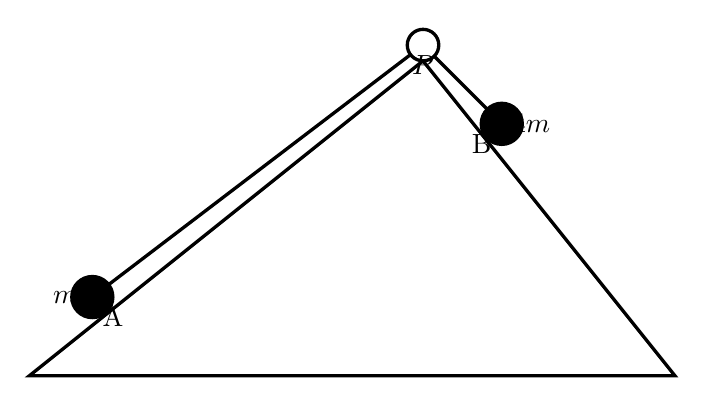
\begin{tikzpicture}
			\coordinate (P1) at (0,0);
			\coordinate (A1) at (-5,-4);
			\coordinate (B1) at (16/5,-4);
			\coordinate (P) at (0,0.2);
			\coordinate (A) at (-4-0.2,-4+4/5+0.2);
			\coordinate (B) at (1,-0.8);
			
			\draw[very thick] (A1)--(P1)--(B1)--cycle;
			\draw[very thick] (A)--(P)--(B);
			
			\draw[very thick,fill=white] (P) circle (0.2);
			\fill (A) circle (.282);
			\fill (B) circle (.282);
			
			\node at (P) [below=0.4] {$P$};
			\node at (A) [below right=0.2] {A};
			\node at (B) [below left=0.2] {B};
			
			\node at (A) [left=0.2] {$m\,\unit{\kg}$};
			\node at (B) [right=0.2] {$4m\,\unit{\kg}$};
			
		\end{tikzpicture}
		
		\begin{parts}
			\part[6][12] Show that when $A$ is released it accelerates 
			towards the pulley at 
			$\frac{7\grav}{15}\,\unit{\m\per\s\squared}$.
			\part[2][4] Assuming that $A$ does not reach the pulley, show that it has moved a distance of $\frac{1}{4}\,\unit{\m}$ when its speed is $\sqrt{\frac{7\grav}{30}}\,\unit{\m\per\s}$.
		\end{parts}
	
		\solnor{
			\begin{parts}
				\part Resolve perpendicular to $\Pi_1$ to get $R=m\grav\cos\alpha=\frac{4}{5}m\grav$ \exmark[B1]
			
				Since $A$ is in motion, $F=\mu R=\frac{1}{3}\frac{4}{5}m\grav=\frac{4}{15}m\grav$ \exmark[B1]
			
				Resolve parallel to both planes \exmark[M1A1]
				\begin{align*}
					ma&=T-\frac{13m\grav}{15} \\
					4ma&=-T+\frac{16m\grav}{5}
				\end{align*}
		
				Solve the simultaneous equations to find $a$ in terms of $\grav$ \exmark[M1E1AG]
				
				\part Use $v^2=u^2+2as$ so $\frac{7\grav}{30}=2\times\frac{7\grav}{15}\times s$ \exmark[M1]
				
				So $s=\frac{1}{4}$ \exmark[E1AG]
			\end{parts}
		}
        \solnpage
        \solnpage
	\end{questions}
%\answerbook
\end{document}